%% Простая презентация с примером включения программного кода и
%% пошаговых спецэффектов
\documentclass[aspectratio=169]{beamer}
\usetheme{SPbAU}
%\useoutertheme{infolines}
\usepackage{fontspec}
\usepackage{xunicode}
\usepackage{xltxtra}
\usepackage{xecyr}
\usepackage{hyperref}
\setmainfont[Mapping=tex-text]{DejaVu Serif}
\setsansfont[Mapping=tex-text]{DejaVu Sans}
\setmonofont[Mapping=tex-text]{DejaVu Sans Mono}
\usepackage{polyglossia}
\setdefaultlanguage{russian}
\usepackage{graphicx}
\usepackage[outputdir=out]{minted}
\usepackage{multicol}
\usepackage{array}
\usepackage{svg}
\usepackage[table]{xcolor}
\usepackage{multirow}

\usepackage{listings}
\setminted[c++]{
  linenos=true,
  fontsize=\footnotesize
}
\lstdefinestyle{mycode}{
  belowcaptionskip=1\baselineskip,
  breaklines=true,
  xleftmargin=\parindent,
  showstringspaces=false,
  basicstyle=\footnotesize\ttfamily,
  keywordstyle=\bfseries,
  commentstyle=\itshape\color{gray!40!black},
  stringstyle=\color{red},
  numbers=left,
  numbersep=5pt,
  numberstyle=\tiny\color{gray},
}
\lstset{escapechar=@,style=mycode}

\definecolor{myred}{RGB}{255, 0, 0}
\definecolor{myblue}{RGB}{0, 0, 255}
\definecolor{myviolet}{RGB}{142, 0, 255}


\setbeamertemplate{navigation symbols}{} % Убрать навигацию

\begin{document}
\title[Комбинаторы запросов к графам]
{
  Разработка библиотеки комбинаторов запросов к графам
}
\author[Шушаков Д.С.]
{
Шушаков Даниил Сергеевич\\
{\footnotesize\textcolor{gray}{Научный руководитель: Григорьев Семен Вячеславович}}\\
}
\institute{Университет ИТМО}


\date{\today}
\frame{\titlepage\thispagestyle{empty}}

\setlength{\parskip}{0.25cm}


%=============================================

\begin{frame}{Графовое представление данных}
  \begin{itemize}
    \item Данные могут представляться в виде графа
    \item Хранятся в графовых базах данных
    \item Вершины и ребра могут иметь свойства вида <<ключ: значение>>
  \end{itemize}

  \center{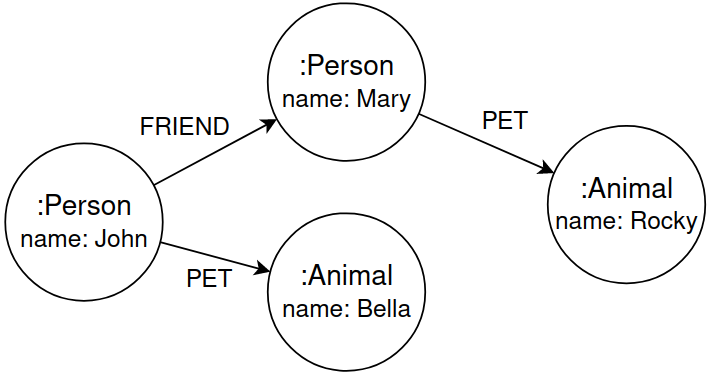
\includegraphics[scale=0.4]{images/gr_example2.png}}
\end{frame}


%=============================================

\begin{frame}[fragile]{Языки запросов}
  \begin{itemize}
    \item Для доступа к данным используются языки запросов, например, Cypher для Neo4j\footnote{https://neo4j.com/docs/getting-started/get-started-with-neo4j/graph-database}
    \item В пользовательском коде они могут использоваться как строки:
          \begin{minted}[frame=single,framesep=10pt, fontsize=\small]{java}
tx.execute("MATCH (n {name: 'my node'}) RETURN n, n.name")
\end{minted}
    \item Недостатки:
          \begin{itemize}
            \item Отсутствие проверки корректности запроса на этапе компиляции
            \item Сложность составления и переиспользования подзапросов
          \end{itemize}
    \item Удобно иметь бесшовную интеграцию запросов в язык программирования
  \end{itemize}

  % Result result = tx.execute( "MATCH (n {name: 'my node'}) RETURN n, n.name" ) )
\end{frame}


%=============================================

\begin{frame}[fragile]{Применение парсер-комбинаторов к графам}

  \begin{columns}[c]
    \begin{column}{0.45\textwidth}
      \begin{itemize}
        \item Запрос к графу --- нахождение путей, удовлетворяющих ограничениям
        \item Ограничения на пути можно описать с помощью грамматики
        \item Грамматику в ЯП общего назначения удобно описать через парсер-комбинаторы
      \end{itemize}
    \end{column}
    \begin{column}{0.58\textwidth}
      \center{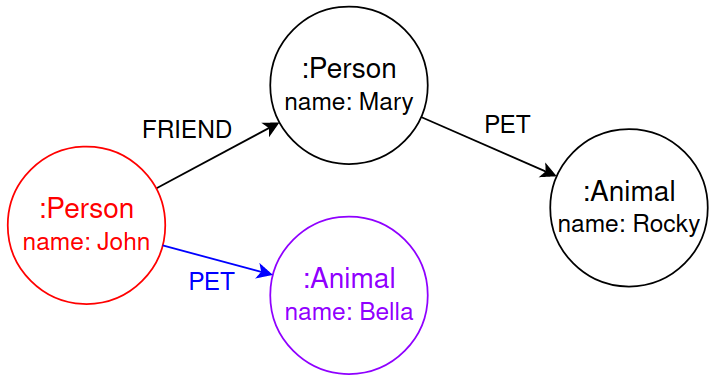
\includegraphics[scale=0.43]{images/gr_query.png}}
      \begin{minted}[frame=single,fontsize=\small, escapeinside=||]{text}
val john = v { it.name == "John" }
val pet = outE { it.label == "PET" }
val s = |\textcolor{myred}{john}| seq |\textcolor{myblue}{pet}| seq |\textcolor{myviolet}{outV()}|
\end{minted}

    \end{column}
  \end{columns}

\end{frame}

%=============================================

\begin{frame}[fragile]{Дополнительные требования}
  \begin{itemize}
    \item Описывать КС-ограничения: существуют применения в области биоинформатики\footnote[1]{Sevon et al (2016). Subgraph Queries by Context-free Grammars}, статическом анализе\footnote[2]{Reps (1997). Program analysis via graph reachability} и т.д.
    \item Разбирать циклы: результатов может быть бесконечно много
  \end{itemize}
  \begin{center}
    \center{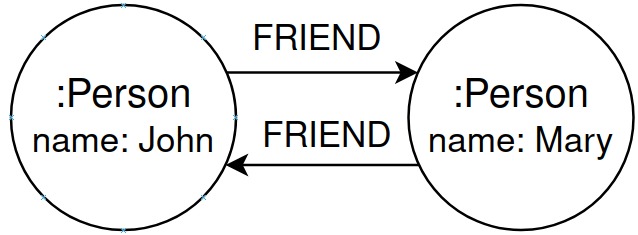
\includegraphics[scale=0.35]{images/gr_friend_loop.png}}
  \end{center}
  %   \begin{minted}[frame=single,fontsize=\small]{kotlin}
  % val s = friend or (s seq friend)
  % \end{minted}
\end{frame}


%=============================================

\begin{frame}{Аналоги}
  \begin{table}[h]
    \renewcommand{\arraystretch}{1.3}
    \begin{tabular}{|b{0.25\linewidth}|b{0.33\linewidth}|b{0.33\linewidth}|}
      \hline
      \textbf{Свойства} & \textbf{Trails\footnote[1]{Kr\"{o}ni et al (2013). Parsing graphs: applying parser combinators to graph traversals}} & \textbf{Meerkat\footnote[2]{\href{https://dl.acm.org/doi/10.1145/2847538.2847539}
          {Izmaylova et al (2016). Practical, General Parser Combinators}}} \\
      \hline
      Сложность      & Экспоненциальная                  & Полиномиальная \\
      \hline
      Левая рекурсия & Нет                               & Да \\
      \hline
      Циклы в графе  & Ограничено                        & Да \\
      \hline
      Типизация      & Контролирует корректность парсера & Возможны некорректные парсеры \\
      \hline
      ЯП             & Scala                             & Scala \\
      \hline
    \end{tabular}
  \end{table}
\end{frame}



%=============================================

\begin{frame}{Подходы к реализации}
  \begin{enumerate}
    \item Meerkat основан на подходах из статьи Practical, General Parser Combinators\footnote[1]{\href{https://dl.acm.org/doi/10.1145/2847538.2847539}
            {Izmaylova et al (2016). Practical, General Parser Combinators}}
          \begin{enumerate}
            \item Мемоизация результатов парсера --- левой рекурсия в грамматиках
            \item Генерация сжатого представления деревьев разбора (SPPF) --- циклы в графах и полиномиальное время
          \end{enumerate}
    \item Trails имеет удобные комбинаторы, контролирующие корректность парсеров
  \end{enumerate}
  % \begin{enumerate}
  %   \item Meerkat основан на подходах из статьи\footnote[1]{Izmaylova et al (2016). Practical, General Parser Combinators}
  %   \item Для поддержки левой рекурсии в грамматиках добавляется мемоизация результатов парсера
  %   \item В процессе разбора генерируется сжатое представление деревьев разбора (SPPF)
  %   \item Оба подхода позволяют получить:
  %         \begin{enumerate}
  %           \item Полиномиальное время работы
  %           \item Поддержку циклов в графе
  %         \end{enumerate}
  % \end{enumerate}
\end{frame}



%=============================================

\begin{frame}{Цель и задачи}
  \textbf{Цель:} разработать библиотеку комбинаторов запросов к графам на основе алгоритмов, предложенных в работе Practical, General Parser Combinators, позволяющую описывать корректные парсеры.

  \textbf{Задачи:}
  \begin{enumerate}
    \item Разработать базовую структуру парсера и комбинаторов с корректной типизацией
    \item Поддержать левую рекурсию в грамматике
    \item Поддержать разбор циклов в графе
    \item Сравнить скорость работы с другими решениями
  \end{enumerate}
\end{frame}


%=============================================

\begin{frame}[fragile]{Реализация: базовая структура парсера}
  Решение разработано на языке Kotlin.
  \begin{minted}[frame=single,framesep=10pt, fontsize=\small]{kotlin}
type Parser = (In) -> ParserResult<Out, Res>
  \end{minted}
  \begin{itemize}
    \item Парсер принимает входящее состояние, возвращает множество выходящий состояний и результатов
    \item Состояние: вершина, ребро, стартовое
    \item Базовые парсеры: \texttt{v, edge, inE, outE, inV, outV}
    \item Комбинаторы: \texttt{seq, or, many и т.д.}
    \item Комбинаторы запрещают объединять парсеры с конфликтующими типами состояний
  \end{itemize}

  %   \begin{minted}[frame=single, fontsize=\small]{kotlin}
  % val person = v()
  % val loves = outE { it.label == "loves" }
  % val friend = outE { it.label == "friend" }
  % val p = person seq ((friend or loves) seq outV()).some
  %   \end{minted}
\end{frame}



%=============================================

\begin{frame}[fragile]{Левая рекурсия: мемоизация результатов}
  \begin{itemize}
    \item Разбор может бесконечно выполняться: левая рекурсия

    \item Хотим, чтобы вычисление парсера исполнялось один раз

    \item Парсер в качестве результата теперь возвращает вычисление:
          \begin{minted}[frame=single,framesep=4pt, fontsize=\small, escapeinside=||]{text}
type Parser = (In) -> (Continuation|\footnote[1]{Можно воспринимать как callback}|<Out, Res>) -> Unit
\end{minted}
    \item Парсер мемоизирует вычисления для каждого входящего состояния

    \item Вычисление запоминает все результаты и продолжения, при появлении нового результата вызывает эти продолжения

    \item Всем продолжениям будет переданы все результаты вычисления

  \end{itemize}
\end{frame}


%=============================================

\begin{frame}{Циклы в графе: генерация SPPF}
  \begin{columns}[c]
    \begin{column}{0.55\textwidth}
      \begin{itemize}
        \item Разбор графа с циклами потенциально может генерировать бесконечно много результатов
        \item Нужно представить результат такого разбора в виде конечной структуры --- SPPF
        \item Результаты из SPPF извлекаются обходом
      \end{itemize}

      \vspace{1cm}

      \begin{minipage}[t]{0.49\textwidth}
        \center{\Large $S \to \varepsilon\ |\ S\ a\ x$}

        \centering Грамматика
      \end{minipage}
      \begin{minipage}[t]{0.49\textwidth}
        \center{\includesvg[inkscapelatex=false,width=0.55\textwidth]{images/gr_loop.svg}}

        \centering Граф-петля
      \end{minipage}%

    \end{column}
    \begin{column}{0.55\textwidth}
      \center{\includesvg[inkscapelatex=false,width=0.75\textwidth]{images/loop.svg}}

      \centering Полученный SPPF
    \end{column}
  \end{columns}
\end{frame}


%=============================================

\begin{frame}[fragile]{Набор данных для исследования времени работы}
  \begin{itemize}
    \item Для исследования добавлена поддержка базы данных Neo4j
    \item Взяты три набора данных: онтологии\footnote[1]{Zhang et al (2016). Context-free path queries on RDF graphs}, SFPQ\_Data\footnote[2]{https://formallanguageconstrainedpathquerying.github.io/CFPQ\_Data/graphs}, Yago\footnote[3]{https://gitlab.inria.fr/tyrex-public/rlqdag}
    \item Для первых двух использовался одинаковый КС-запрос
          \begin{minted}[frame=single,fontsize=\small, escapeinside=||]{text}
|$Q_1 \to subclassof^{-1}\ Q_1?\ subclassof$|
|$Q_1 \to type^{-1}\ Q_1?\ type$|
\end{minted}
    \item Для Yago использовался регулярный запрос
          \begin{minted}[frame=single,fontsize=\footnotesize]{text}
MATCH 
(x)-[:P1]->()-[:P2]->()-[:P3*1..]->()-[:P4*1..]->(:Entity{id:'42'}) 
RETURN DISTINCT x
\end{minted}
          % MATCH (x)-[:P74636308]->()-[:P59561600]->()-[:P13305537*1..]->
          % ()-[:P92580544*1..]->(:Entity{id:'40324616'}) RETURN DISTINCT x
  \end{itemize}

\end{frame}


%=============================================

\begin{frame}{Результаты исследования времени работы}
  \vspace*{-0.9\baselineskip}
  \begin{table}[h]
    \renewcommand{\arraystretch}{1.3}
    \begin{tabular}{|b{0.02\linewidth}|b{0.21\linewidth}|b{0.15\linewidth}|b{0.15\linewidth}|>{\columncolor{yellow!20}}b{0.15\linewidth}|b{0.14\linewidth}|}
      \hline
      \multicolumn{2}{|c|}{\textbf{Граф}}        & \textbf{Кол-во вершин}    & \textbf{Кол-во рёбер} & \textbf{Мое реш. (мс)} & \textbf{Meerkat (мс)} \\
      \hline
      \multirow{4}{*}{\rotatebox{90}{онтологии}} & atom-primitive            & 291        & 685        & \textbf{19.5} & 22.0 \\
                                                 & b.-m.-p.\footnote[1]{biomedical-mesure-primitive} & 341        & 711        & \textbf{23.5} & 42.5 \\
                                                 & generations               & 129        & 351        & \textbf{1.3}  & 1.4 \\
                                                 & pizza                     & 671        & 2,604      & \textbf{61.4} & 123.9 \\
      \hline

      \multirow{4}{*}{\rotatebox{90}{SFPQ\_Data}} & enzyme                    & 48,815     & 86,543     & 121           & \textbf{116} \\
                                                 & eclass                    & 239,111    & 360,248    & 1220          & \textbf{1095} \\
                                                 & go                        & 582,929    & 1,437,437  & 6231          & \textbf{5367} \\
                                                 & go\_hierarchy             & 45,007     & 490,109    & 12015         & \textbf{8337} \\
      \hline
      \multicolumn{1}{|l}{}                      & \multicolumn{1}{l|}{yago} & 42,832,856 & 62,643,951 & \textbf{5558} & OOM \\
      \hline
    \end{tabular}
  \end{table}
\end{frame}



%=============================================

\begin{frame}{Результаты}
  \begin{itemize}
    \item Разработаны базовая структура парсера и комбинаторов, проверяющая корректность во время компиляции
    \item Поддержаны леворекурсивные грамматики
    \item Поддержан разбор циклов в графе
    \item Реализована базовая поддержка Neo4j графов
    \item Проведено исследование времени работы в сравнении с Meerkat:
          \begin{itemize}
            \item На первом датасете мое решение быстрее в среднем на 28\%
            \item На втором датасете Meerkat быстрее в среднем на 15\%
            \item На третьем датасете только мое решение успешно выполнилось
          \end{itemize}
  \end{itemize}
\end{frame}


% --------- ДОП СЛАЙДЫ -------------
\appendix


\begin{frame}{Аналоги: Meerkat}
  \begin{itemize}
    \item Meerkat --- изначально библиотека с комбинаторами для разбора текста, реализующий алгоритм из статьи \footnote[1]{\href{https://dl.acm.org/doi/10.1145/2847538.2847539}
            {Izmaylova et al (2016). Practical, General Parser Combinators}}
    \item В последствии расширена поддержкой запросов к графам\footnote[2]{Verbitskaia et al (2018). Parser combinators for context-free path querying}
    \item Т.к. изначально разрабатывалась для разбора текста, в ней парсеры принимали позицию в тексте
    \item В расширении позиция в тексте семантически поменялась на номер вершины в графе
  \end{itemize}
\end{frame}

\begin{frame}[fragile]{Сигнатуры комбинаторов}

  \begin{minted}[frame=single,fontsize=\footnotesize]{kotlin}
fun BaseParser<I, O1, R1>.seq(p2: BaseParser<O1, O2, R2>)
    : BaseParser<I, O2, Pair<R1, R2>>

fun BaseParser<I, O, R>.or(p2: BaseParser<I, O, R>)
    : BaseParser<I, O, R>

fun rule(first: BaseParser<I, O, R>, vararg rest: BaseParser<I, O, R>)

fun BaseParser<I, O, A>.using(f: (A) -> B): BaseParser<I, O, B>

fun BaseParser<I, O, R>.that(constraint: BaseParser<O, O2, R2>)
    : BaseParser<I, O, R> 
    
val BaseParser<S, S, R>.many: BaseParser<S, S, List<R>>
val BaseParser<S, S, R>.some: BaseParser<S, S, List<R>>
\end{minted}
\end{frame}


\begin{frame}[fragile]{Комбинаторы that и using}
  Использование комбинаторов \texttt{that, using}:
  \begin{minted}[frame=single, fontsize=\small]{kotlin}
val mary = outV { it.value == "Mary" }
val loves = outE { it.label == "loves" }
val friend = outE { it.label == "friend" }
val maryLover = v().that(loves seq mary)
val p = maryLover seqr (friend seq outV()).some
val s = p using {edges -> Pair(edges.size, edges.last().second)}
\end{minted}
\end{frame}


\begin{frame}[fragile]{Запросы для исследования времени (КС)}
  \begin{minted}[frame=single, fontsize=\footnotesize]{kotlin}
val subclassof1 = throughInE { it.label == "subClassOf" }
val subclassof = throughOutE { it.label == "subClassOf" }
val type1 = throughInE { it.label == "type" }
val type = throughOutE { it.label == "type" }
val Q1 = LazyParser<Neo4jVertexState, Neo4jVertexState, Any>()
Q1.p = (subclassof1 seq (Q1 or eps()) seq subclassof) or
        (type1 seq (Q1 or eps()) seq type)
\end{minted}
  \begin{minted}[frame=single, fontsize=\footnotesize]{scala}
val subclassof1: Symbol[L, N, _] = inE("subClassOf")
val subclassof: Symbol[L, N, _] = outE("subClassOf")
val type1: Symbol[L, N, _] = inE("type")
val _type: Symbol[L, N, _] = outE("type")
val grammar: Symbol[L, N, _] = 
  syn((subclassof1 ~ syn(grammar | ε) ~ subclassof) |
    (type1 ~ syn(grammar | ε) ~ _type))
\end{minted}


\end{frame}


\begin{frame}[fragile]{Запросы для исследования времени (yago)}


  \begin{minted}[frame=single,fontsize=\footnotesize]{kotlin}
(v { it.properties["id"] == "40324616" } seq
(inE { it.label == "P92580544" } seq inV()).some seq
(inE { it.label == "P13305537" } seq inV()).some seq
inE { it.label == "P59561600" } seq inV() seq
inE { it.label == "P74636308" } seq inV())
\end{minted}

  \begin{minted}[frame=single, fontsize=\footnotesize]{scala}
syn(V((e: Entity) => e.getProperty("id") == "40324616") ~
inE((e: Entity) => e.label() == "P92580544").+ ~
inE((e: Entity) => e.label() == "P13305537").+ ~
inE((e: Entity) => e.label() == "P59561600") ~
inE((e: Entity) => e.label() == "P74636308"))
  \end{minted}

\end{frame}






\end{document}

